\section{计算成本}
\label{sec:budget-costs}

式~\eqref{eq:budget-mse-cost-product}说明，无偏方法之间比较的是“单样本方差乘单样本成本”。可是“一个样本”在不同方法里含义不同：拒绝采样的一个输出要先生成并淘汰若干候选，Markov链每步都产生一个状态但相邻状态高度相关，有的方法在抽第一个样本之前就要做一次矩阵分解或一轮试运行。要让比较公平，就要把这些开销记在同一本账上，并且明确“成本”是按什么单位计的。

\paragraph{成本的组成}
一次随机计算的开销可以分成三类。第一类是每次迭代的操作：生成基础随机数，按建议分布生成候选，计算目标密度、密度比或梯度，计算被积函数。第二类把迭代换算成输出：拒绝采样平均要做若干次迭代才输出一个样本，抽稀的链每$k$步才保存一个状态。第三类只发生一次或每条链一次：矩阵分解、试运行与建议分布的拟合、控制系数或分层方案的预估，以及链开始时为摆脱初值而舍弃的$b$步。

记一次迭代的成本为$c_{\mathrm{it}}$，一个输出样本的成本为$c_{\mathrm{out}}$，一次性开销为$C_{0}$。输出$n$个样本的总成本是
\begin{equation}
  C=C_{0}+b\,c_{\mathrm{it}}+n\,c_{\mathrm{out}} .
  \label{eq:budget-total-cost}
\end{equation}
图~\ref{fig:budget-cost-ledger}把这几项的关系画成一张账：单项操作合成一次迭代，迭代乘以候选数或抽稀间隔得到输出样本，输出样本再乘以相关性的影响得到下文的有效样本。计成本的单位可以是运行时间，也可以是某种主导操作的次数（如目标密度的计算次数）。用操作次数便于复现和推导，用时间更贴近实际，二者在向量化、缓存或并行时可能给出不同的排序，比较前要说明用的是哪一种。

\begin{BookInlineFigure}
  \centering
  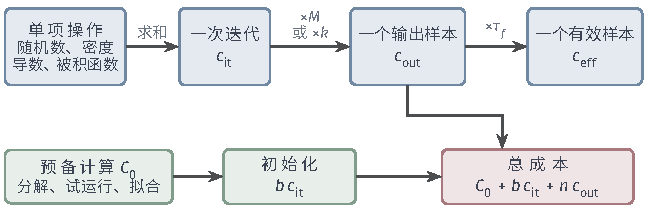
\includegraphics[width=110mm]{figures/07-probability/08-sampling-and-integration/tikz/budget-cost-ledger/figure.pdf}
  \caption{一次随机计算的成本账。上排是按单位累积的成本：单项操作合成一次迭代$c_{\mathrm{it}}$，拒绝采样乘以平均候选数$M$、抽稀乘以间隔$k$得到一个输出样本$c_{\mathrm{out}}$，相关链再乘以$\tau_{f}$得到针对被积函数$f$的一个有效样本。下排是只计一次的开销：预备计算$C_{0}$和每条链初始化舍弃的$b$步，它们与$n$个输出的成本合成总成本~\eqref{eq:budget-total-cost}。}
  \label{fig:budget-cost-ledger}
\end{BookInlineFigure}

\paragraph{工作量归一化方差}
设某个无偏方法的输出相互独立，单样本方差为$\sigma^{2}$，单样本成本为$c$，一次性开销为$C_{0}$，暂不考虑初始化。总预算$C>C_{0}$可买$n=(C-C_{0})/c$个样本（忽略取整），估计的方差为
\begin{equation}
  \operatorname{Var}(\hat{I})=\frac{\sigma^{2}c}{C-C_{0}} .
  \label{eq:budget-var-budget}
\end{equation}
称$\sigma^{2}c$为\term{工作量归一化方差}（work-normalized variance）。预算远大于$C_{0}$时，它是比较两种方法的唯一量：方法甲优于方法乙，当且仅当$\sigma_{\text{甲}}^{2}c_{\text{甲}}<\sigma_{\text{乙}}^{2}c_{\text{乙}}$。单看方差或单看成本都会误判：方差小一半而每个样本贵三倍的方法，在同样预算下反而更差。

一次性开销使比较依赖预算。设方法乙没有预备开销，方法甲有$C_{0}>0$且$\sigma_{\text{甲}}^{2}c_{\text{甲}}<\sigma_{\text{乙}}^{2}c_{\text{乙}}$。由式~\eqref{eq:budget-var-budget}，甲的方差较小当且仅当
\[
  \frac{\sigma_{\text{甲}}^{2}c_{\text{甲}}}{C-C_{0}}<\frac{\sigma_{\text{乙}}^{2}c_{\text{乙}}}{C},
\]
整理得
\begin{equation}
  C>C_{\times}=\frac{C_{0}\,\sigma_{\text{乙}}^{2}c_{\text{乙}}}{\sigma_{\text{乙}}^{2}c_{\text{乙}}-\sigma_{\text{甲}}^{2}c_{\text{甲}}} .
  \label{eq:budget-crossover}
\end{equation}
预算低于$C_{\times}$时，花在准备上的成本收不回来。

以第~\ref{chap:variance-reduction}章的尾概率为例。直接平均的$\sigma^{2}=I(1-I)\approx0.01798$，每个样本成本记为$1$；从$\operatorname{Exp}(1/4)$抽样的重要性采样单样本方差约$0.001749$，每个样本成本记为$1.5$，选定建议分布的预备开销记为$C_{0}=2000$。两者的工作量归一化方差分别为
\[
  0.01798\times1=0.01798,\qquad0.001749\times1.5\approx0.002623,
\]
大预算下重要性采样约好$6.9$倍。代入式~\eqref{eq:budget-crossover}，
\[
  C_{\times}=\frac{2000\times0.01798}{0.01798-0.002623}\approx2342 .
\]
本章开头的预算$10^{5}$远超过它，准备是值得的。

\paragraph{拒绝候选与矩阵分解}
拒绝采样的每个候选被接受的概率是$1/M$，$M$为包络常数（第~\ref{chap:sample-generation}章）。各候选独立，所以得到一个输出所需的候选数$N$服从参数$1/M$的几何分布，$\mathbb{P}(N=j)=(1-1/M)^{j-1}/M$，其均值为
\[
  \mathbb{E}[N]=\sum_{j\ge1}j\Bigl(1-\frac1M\Bigr)^{j-1}\frac1M=\frac{1/M}{(1/M)^{2}}=M .
\]
若每个候选要生成一次建议样本（成本$c_{q}$）、计算一次接受判据（成本$c_{\mathrm{acc}}$），被接受的样本还要计算一次被积函数（成本$c_{f}$），则
\begin{equation}
  c_{\mathrm{out}}=M\,(c_{q}+c_{\mathrm{acc}})+c_{f} .
  \label{eq:budget-rejection-cost}
\end{equation}
被淘汰的候选不产生输出，但其成本全额计入。$M$随维数增长时，这一项可能成为全部成本的主体。

生成$\mathcal{N}(\bm{\mu},\bm{\Sigma})$的样本时，要先把$d\times d$的协方差矩阵分解为$\bm{\Sigma}=\bm{L}\bm{L}^{\top}$，此后每个样本是$\bm{\mu}+\bm{L}\bm{Z}$。按\BookChapterRef{chap:direct-linear-solvers}{卷二第12章“线性方程的直接求解”}，Cholesky分解约需$d^{3}/3$次乘加，下三角矩阵乘向量约需$d^{2}$次。抽$n$个样本时，平均到每个样本的乘加次数约为
\[
  \frac{d^{3}/3}{n}+d^{2}=d^{2}\Bigl(1+\frac{d}{3n}\Bigr).
\]
$n$远大于$d$时分解的开销可以忽略；$n$与$d$相当或更小时（例如$d=1000$只抽$100$个样本），分解占了大部分成本，这时比较方法必须把$C_{0}$计入，而不能只看每个样本的$d^{2}$。

\paragraph{迭代、输出样本与有效样本}
Markov链每步输出一个状态，相邻状态相关，保存下来的状态数不能直接当作样本数。设链平稳，被积函数$f$的单步方差为$\gamma_{0}$，长期方差为$\sigma_{\mathrm{LR}}^{2}$，记
\begin{equation}
  \tau_{f}=\frac{\sigma_{\mathrm{LR}}^{2}}{\gamma_{0}},\qquad N_{\mathrm{eff}}=\frac{N}{\tau_{f}} .
  \label{eq:budget-tau}
\end{equation}
这里的$N_{\mathrm{eff}}$就是第~\ref{chap:monte-carlo-integration-error}章的有效样本量：$N$步相关平均的渐近方差$\sigma_{\mathrm{LR}}^{2}/N$等于$N_{\mathrm{eff}}$个独立样本的方差$\gamma_{0}/N_{\mathrm{eff}}$。于是忽略初始化时，针对$f$的一个有效样本的成本是
\begin{equation}
  c_{\mathrm{eff}}=c_{\mathrm{it}}\,\tau_{f},
  \label{eq:budget-eff-cost}
\end{equation}
相关链的工作量归一化方差是
\[
  \gamma_{0}\,c_{\mathrm{eff}}=\gamma_{0}c_{\mathrm{it}}\tau_{f}=\sigma_{\mathrm{LR}}^{2}c_{\mathrm{it}} .
\]

$\tau_{f}$属于“链与被积函数”这一对，而不是只属于链。以平稳自回归链
\begin{equation}
  X^{(t+1)}=\rho X^{(t)}+\sqrt{1-\rho^{2}}\,\varepsilon^{(t)},\qquad\varepsilon^{(t)}\sim\mathcal{N}(0,1)\ \text{独立}
  \label{eq:budget-ar1}
\end{equation}
为例，目标$\mathcal{N}(0,1)$。对$f(x)=x$，$\gamma_{k}=\rho^{k}$；对$f(x)=x^{2}$，$\gamma_{k}=2\rho^{2k}$。分别对几何级数求和，得到
\[
  \tau_{x}=\frac{1+\rho}{1-\rho},\qquad\tau_{x^{2}}=\frac{1+\rho^{2}}{1-\rho^{2}} .
\]
$\rho=0.9$时$\tau_{x}=19$，$\tau_{x^{2}}\approx9.53$：同一条链的同一段记录，估计$\mathbb{E}[X^{2}]$时的有效样本数约是估计$\mathbb{E}[X]$时的两倍。图~\ref{fig:budget-ess-thinning}(a)画出每步的有效样本数$1/\tau_{f}$随$\rho$的变化。

\begin{BookInlineFigure}
  \centering
  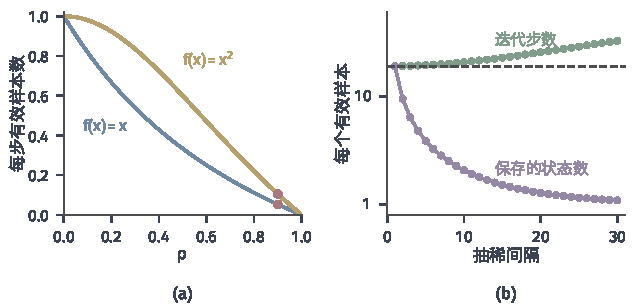
\includegraphics[width=108mm]{figures/07-probability/08-sampling-and-integration/matplotlib/budget-ess-thinning/figure.pdf}
  \caption{平稳自回归链（目标$\mathcal{N}(0,1)$）的有效样本。(a)~每步迭代提供的有效样本数$1/\tau_{f}$：蓝线$f(x)=x$，黄线$f(x)=x^{2}$，红点为$\rho=0.9$。(b)~$\rho=0.9$、$f(x)=x$时每隔$k$步保存一个状态：绿线为每个有效样本所需的迭代步数，紫线为所需保存的状态数，深灰虚线为不抽稀时的$19$步。}
  \label{fig:budget-ess-thinning}
\end{BookInlineFigure}

保存时常做\term{抽稀}（thinning）：每$k$步只保存一个状态。抽稀后的序列仍是自回归链，系数为$\rho^{k}$，长度为$N/k$。对$f(x)=x$，每个有效样本需要保存$(1+\rho^{k})/(1-\rho^{k})$个状态，相应的迭代步数是
\[
  k\,\frac{1+\rho^{k}}{1-\rho^{k}} .
\]
$\rho=0.9$、$k=10$时，前者约$2.07$，后者约$20.7$，比不抽稀的$19$步还多。图~\ref{fig:budget-ess-thinning}(b)显示了这一点：抽稀减少存储，不减少计算，对这个例子还略微损失精度。只有被积函数本身很贵，例如每次求值的成本$c_{f}$远大于一步转移的成本时，抽稀才能节省计算，因为这时每个保存状态的成本是$k\,c_{\mathrm{it}}+c_{f}$，适当的$k$可以减少昂贵的求值次数。

链的初始化另有成本。每条链舍弃前$b$步，花费$b\,c_{\mathrm{it}}$，这一项不随保存的样本数摊薄，启动的链越多，总的初始化成本越高。第~\ref{sec:budget-allocation}节比较多次启动与单链延长时会用到这一点。

\paragraph{三种采样方式的成本比较}
把上面的账用到第~\ref{chap:sample-generation}章的双峰混合
\[
  \pi=0.3\,\mathcal{N}(-2,0.5^{2})+0.7\,\mathcal{N}(2,1)
\]
上，被积函数取$f(x)=x$。这时
\[
  I=0.3\times(-2)+0.7\times2=0.8,\qquad\operatorname{Var}_{\pi}(f)=0.3\times4.25+0.7\times5-0.8^{2}=4.135 .
\]

作为教学约定，取成本单位：一个均匀数记$1$，一个标准高斯数记$2$，计算一次混合密度记$4$（两个指数），计算一次单个高斯包络的密度记$2$，计算一次$f$记$1$。三种方式的单样本成本如下。
\begin{itemize}
  \item 分步生成：先用一个均匀数选成分，再生成一个高斯数，最后算$f$，$c_{\mathrm{out}}=1+2+1=4$，样本独立，$\tau_{f}=1$。
  \item 拒绝采样：在网格上选使$M$最小的高斯包络，得到$\mathcal{N}(0.25,2.2^{2})$，$M\approx2.29$，接受率约$0.44$。每个候选要一个高斯数、一次包络密度、一次目标密度和一个均匀数，共$9$，由式~\eqref{eq:budget-rejection-cost}，$c_{\mathrm{out}}\approx9\times2.29+1\approx21.7$。
  \item 随机游走Metropolis：每步一个高斯数、一次目标密度、一个均匀数和一次$f$，$c_{\mathrm{it}}=8$。$\tau_{f}$由$10^{6}$步链的分块均值估计，步长$s=1,2.5,4$时分别约为$66$、$8.5$、$6.5$。
\end{itemize}

由式~\eqref{eq:budget-eff-cost}，Metropolis每个有效样本的成本分别约为$527$、$68$、$52$。图~\ref{fig:budget-sampler-costs}(b)把五个数放在对数坐标上：对这个一维目标，分步生成比最好的链便宜十几倍，拒绝采样介于其间。若只按“保存的状态数”比较，Metropolis每步成本$8$只是拒绝采样的约三分之一，结论正好相反。图~\ref{fig:budget-sampler-costs}(a)给出原因：步长$s=1$时，状态要在两个峰之间往返，自相关衰减很慢；步长较大时接受率降低，但跨峰更容易，$\tau_{f}$反而小得多。

\begin{BookInlineFigure}
  \centering
  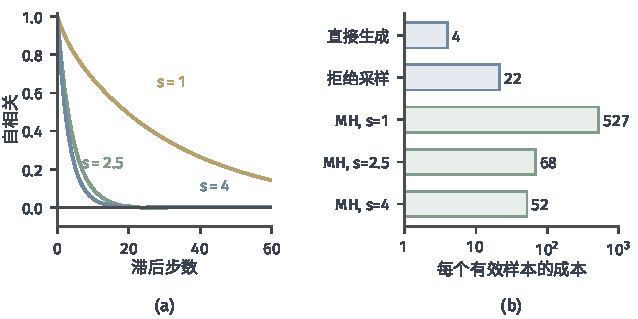
\includegraphics[width=108mm]{figures/07-probability/08-sampling-and-integration/matplotlib/budget-sampler-costs/figure.pdf}
  \caption{双峰混合$0.3\,\mathcal{N}(-2,0.5^{2})+0.7\,\mathcal{N}(2,1)$、$f(x)=x$时三种采样方式的成本（教学约定的操作计数）。(a)~随机游走Metropolis的自相关函数，三条线对应步长$s=1,2.5,4$，各由$10^{6}$步链计算。(b)~每个有效样本的成本：蓝色为独立样本，绿色为Metropolis（每步成本乘以估计的$\tau_{f}$）。}
  \label{fig:budget-sampler-costs}
\end{BookInlineFigure}

这里的$\tau_{f}$是从一段有限记录估计的，它本身有误差，而且只有在链确实走遍两个峰时才可信；第~\ref{sec:budget-stopping}节会看到有限记录可能完全没有发现某个峰。比较结论还依赖成本单位：若目标密度极贵而高斯数几乎免费，各项的比例会改变。账本的作用是让这些假设明确可查，而不是给出与假设无关的排名。
